\section{Efficiency of the Trigger for Event Type Hadron}

The trigger for hadronic events was chosen to be very efficient in
order to make it more easily understood.  The Monte Carlo simulation
predicts a 99.8\% trigger efficiency for $\Upsilon(1S)$ hadronic
decays, and 99.6\% for the $\Upsilon(2S)$ and $\Upsilon(3S)$.  I can
therefore immediately present 0.2\% and 0.4\% upper bounds on the
errors in these predictions, but I will need to do more work to prove
that the true trigger efficiency isn't much lower than this.  One
could imagine hadronic decays failing the trigger which are not
present in the Monte Carlo simulation, or that the real trigger is not
as responsive as the simulation assumes.  The cascades study was able
to limit these possibilities within an error of 1.34\%, but further
reduction is possible with an independent argument.

I will break the argument into two parts.  First, I will extract a
large data sample from the database dataset with the TwoTrack trigger
line to verify the Monte Carlo's prediction of the efficiency of the
CC part of the trigger.  Then I will build a simpler simulation of the
trigger, which I can control, and use this to show that the trigger
efficiency is insensitive to reasonable variations of input.

\subsection{Uncertainty in CC Simulation}

To verify the CC part of the trigger, I define a new event type called
cccheck.  A cccheck event must
\begin{itemize}
  \item satisfy the TwoTrack trigger and \lfourdec,
  \item have two or more quality tracks,
  \item have charged energy $>$ 15\% \ecom,
  \item \dxy\ $<$ 5 mm,
  \item \dz\ $<$ 7.5 cm,
  \item and have \pone\ $<$ 80\% \ebeam.
\end{itemize}
These events are essentially the same as events of type hadron, except
that no CC energy is required, not even in the trigger.  For these
events, I can then ask, ``how many satisfy the analysis trigger
(Hadron or RadTau or ElTrack)?''  If data and Monte Carlo yield the
same result, then the Monte Carlo correctly reproduces the CC part of
the trigger.  The data are continuum-subtracted on-resonance runs from
the database dataset, with a bhabha continuum subtraction as described
in Chapter \ref{chp:datasets}.  The results of this comparison are
presented in Table \ref{trigger_neutraltable}.  Beam-gas and cosmic
ray corrections alter these values negligibly.

\begin{table}[p]
  \caption{\label{trigger_neutraltable} Probability that cccheck
  events pass ``Hadron or RadTau or ElTrack'' in data and Monte
  Carlo.  Uncertainties in Monte Carlo are negligible.}
  \begin{center}
    \begin{tabular}{l c c c}
      & $\Upsilon(1S)$ & $\Upsilon(2S)$ & $\Upsilon(3S)$ \\
      data & 99.45 $\pm$ 0.30\% & 99.01 $\pm$ 0.51\% & 97.67 $\pm$ 1.17\% \\
      Monte Carlo & 99.79\% & 99.76\% & 99.73\% \\
    \end{tabular}
  \end{center}
\end{table}

\begin{figure}[p]
  \begin{center}
    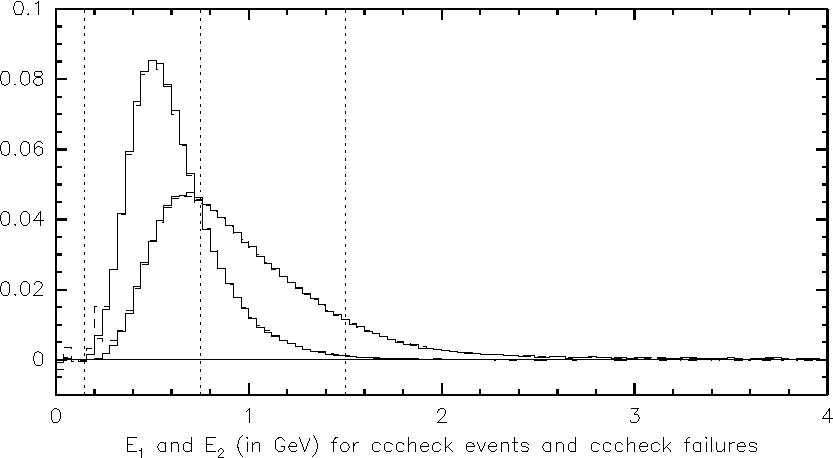
\includegraphics[width=\linewidth]{plots/trigger_neutralpart}
  \end{center}
  \caption{\label{trigger_neutralpart} Biggest and second-biggest
    shower energies in cccheck events (solid) and cccheck failures
    (dashed).  (All cccheck failures satisfy database filters.)  The
    CBLO (0.15 GeV), CBMD (0.75 GeV), and CBHI (1.5 GeV) thresholds
    are indicated by dotted lines.}
\end{figure}

The measured probabilities are in agreement, but their uncertainty is
large for the $\Upsilon(3S)$, which has the largest
continuum-subtraction.  Both the $\Upsilon(2S)$ and $\Upsilon(3S)$ are
open to cascade decays (into $\Upsilon$ and $\chi_b$), so I would
expect their trigger efficiencies to be similar, as it is in the Monte
Carlo.  Therefore, I will apply the $\Upsilon(2S)$ CC trigger
uncertainty to $\Upsilon(3S)$ data and obtain the following errors on
hadronic trigger efficiency: 0.45\% for the $\Upsilon(1S)$, 0.91\% for
the $\Upsilon(2S)$ and $\Upsilon(3S)$.  These errors are sums of the
data--Monte Carlo discrepancies and the data uncertainties in
quadrature.  Another error, from the DR simulation, will be applied to
this.

One might argue that these specially-chosen events have sculpted
shower energy distributions.  This is shown to be not true in Figure
\ref{trigger_neutralpart}: the two biggest showers (which are the only
ones that matter for triggering) have the same distributions in
cccheck events as in other $\Upsilon$ decays.

\subsection{Uncertainty in DR Simulation}

Unfortunately, I cannot perform the same study for the tracking part
of the trigger because no unbiased all-neutral trigger line exists for
CLEO-III.  Instead, I will reproduce the Monte Carlo simulation in a
way that I can control, and vary the input (within uncertainties) to
verify that the trigger response is largely unaffected.

My Toy Monte Carlo has the following algorithm.
\begin{enumerate}

  \item Randomly choose a ``number of quality tracks'' from an input
    distribution.  The distribution from the Full Monte Carlo is
    presented on the far left of Figure \ref{trigger_toymcexamples}.

  \item Randomly choose a ``number of CBLO clusters'' and a ``number
    of CBMD clusters.''  The distributions from which \#CBLO and
    \#CBMD are chosen depend on the given number of quality tracks, to
    try to reproduce some of the correlations exhibited by real
    events.  This is why the number of quality tracks is picked first:
    it best characterizes the event type.  The middle of Figure
    \ref{trigger_toymcexamples} shows two sample \#CBMD distributions,
    one for 0-track events and another for 4-track events.

    The CBLO clusters and CBMD clusters are not correlated with each
    other, but in the Toy Monte Carlo \#CBLO $<$ \#CBMD happens only
    0.18\% of the time.

  \item Randomly choose a ``number of AXIAL tracks.''  This, too,
    depends on the number of quality tracks.  The far right of Figure
    \ref{trigger_toymcexamples} shows the AXIAL track distributions
    given four quality tracks from the Full Monte Carlo and from data.
    By swapping input distributions, I will find the trigger's
    sensitivity to data--Monte Carlo differences.

  \item Randomly choose a ``number of STEREO tracks,'' given a number
    of AXIAL tracks.  This should be tied to AXIAL tracks rather than
    quality tracks to account for the large correlation between these
    two variables.

  \item Construct a trigger decision out of \#CBLO, \#CBMD, \#AXIAL,
    and \#STEREO, and repeat 100,000 times.  This will be
    enough to calculate the trigger efficiency to an uncertainty of
    0.03\%.  All trigger efficiencies quoted from the Toy Monte Carlo
    have this same small uncertainty.

\end{enumerate}

\begin{figure}[t]
  \begin{center}
    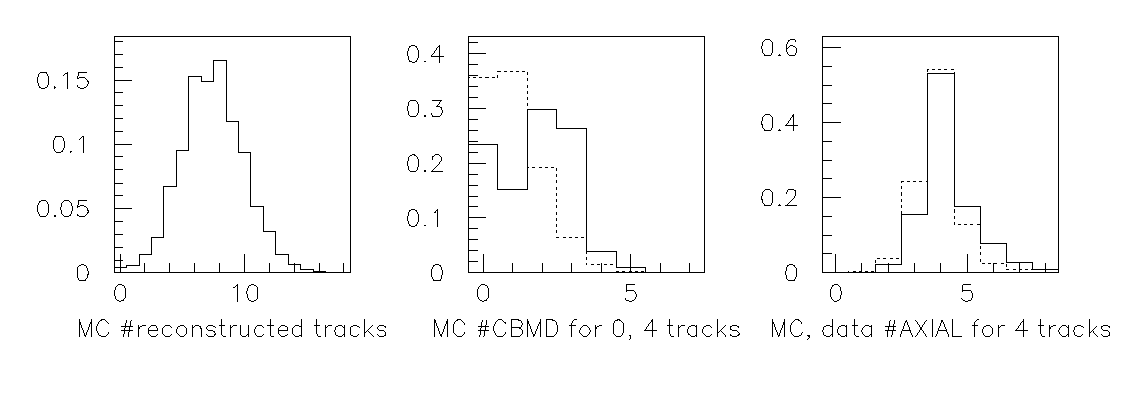
\includegraphics[width=\linewidth]{plots/trigger_toymcexamples}
  \end{center}
  \vspace{-1.3 cm}
  \caption{\label{trigger_toymcexamples} A few sample distributions
    which are used by the Toy Monte Carlo.  Left: \#quality tracks
    from the Full Monte Carlo.  Middle: \#CBMD distributions from the
    Full Monte Carlo, given zero quality tracks (solid) or four
    quality tracks (dotted).  Right: \#AXIAL distributions from the
    Full Monte Carlo (solid) and data (dotted), each for 4 quality
    tracks.}
\end{figure}

All tests will be performed with the Toy Monte Carlo, so differences
in trigger efficiency should be measured relative to the Toy Monte
Carlo with default inputs, not the Full Monte Carlo.  Yet I need to
know how well the Toy Monte Carlo reproduces the Full Monte Carlo, so
this will be my first comparison test.  The default input
distributions (\#quality tracks, \#CBLO, etc.) for the Toy Monte Carlo
are taken from the Full Monte Carlo, so this test only determines how
much is lost by not fully simulating events in the Toy Monte Carlo.
Any difference between the default Toy Monte Carlo and the Full Monte
Carlo will be taken as a systematic error, which will be applied once
to the trigger uncertainty.  The following comparison yields
differences less than 0.14\%.
\begin{center}
  \begin{tabular}{l c c c}
    & $\Upsilon(1S)$ & $\Upsilon(2S)$ & $\Upsilon(3S)$ \\\hline
    Full MC & 99.68\% & 99.44\% & 99.50\% \\
    Toy MC (default) & 99.67\% & 99.54\% & 99.64\% \\
  \end{tabular}
\end{center}

The second test estimates sensitivity to track-finding errors in the
trigger.  While the default Toy Monte Carlo gets its \#AXIAL tracks
and \#STEREO tracks from the Full Monte Carlo, the ``get trigger
tracks from data'' variant uses distributions extracted from raw data.
These raw data were not selected for a particular event type, so they
contain bhabha events as well as hadrons, but only in the two-quality
track column.  These data were also filtered by the trigger itself.
Events with zero AXIAL tracks exist in the sample (from the
BarrelBhabha trigger line) but there are very few one-AXIAL track
events.  Nevertheless, associating AXIAL track distributions with a
hadronic number of quality tracks distribution should unfold these
distortions.

As an alternate method, I derived another \#AXIAL tracks distribution
from the Full Monte Carlo, but tuned it to look like data.  The
\#AXIAL track distributions in data tend toward slightly lower values
than those in the Full Monte Carlo, which is to say that the AXIAL
track finding efficiency is lower in data than it is in Monte Carlo.
For an example of this, see the far right of Figure
\ref{trigger_toymcexamples}; the dotted data distribution is smeared
8.3\% lower than the solid Full Monte Carlo distribution (every
twelfth track is dropped).  To generate this distribution, I apply the
following convolution to the Full Monte Carlo \#AXIAL track
distribution:
\begin{equation}
  t'(n) = \sum_{k=0}^\infty t(n+k)
  \left(\begin{array}{c} n+k \\ n
  \end{array}\right) (1 - p)^n p^k
  \label{trigger_trackconvolutioneqn}
\end{equation}
where $t(n)$ is the number of tracks distribution before convolution,
$t'(n)$ after, and $p$ = 0.083 is the probability of losing one track.
This will place a more stringent bound on the track-finding systematic
since it will always lower the trigger efficiency, unlike the
data-based method (described in the previous paragraph), which has
competing effects.

In both methods, the maximum deviation is 0.18\%.
\begin{center}
  \begin{tabular}{l c c c}
    & $\Upsilon(1S)$ & $\Upsilon(2S)$ & $\Upsilon(3S)$ \\\hline
    Toy MC (default) & 99.67\% & 99.54\% & 99.64\% \\
    Get trigger tracks from data & 99.56\% & 99.42\% & 99.49\% \\
    Drop every 12$^{\mbox{\scriptsize th}}$ AXIAL track from MC & 99.50\% & 99.36\% & 99.47\%
  \end{tabular}
\end{center}

The third and fourth tests estimate sensitivity to charged particle
multiplicity and to track reconstruction efficiency.  As can be seen
in the cascades study (Figure \ref{cascades_tracks}), the Monte Carlo
generally underestimates the number of quality tracks.  This could be
because the Monte Carlo generates too few charged particles or because
the Monte Carlo has too low of a track reconstruction efficiency, or
too many Monte Carlo tracks fail track quality cuts (equivalent to
reconstruction efficiency).  The third test will be to swap the Monte
Carlo's quality track distribution for one from data, and the fourth
test will be to vary the track finding efficiency in the Monte Carlo.

To swap the Monte Carlo's quality track distribution for one from
data, I need only read values off of Figure \ref{cascades_tracks}.
There is one caveat: the $\Upsilon(1S)$ represented in the cascades
study is boosted and can suffer from track confusion with the two
pions.  Therefore, I must first replace the \#quality tracks
distribution from the Full Monte Carlo with one from the cascade Monte
Carlo.  This is also read off of Figure \ref{cascades_tracks}; it is
the solid histogram.

The number of tracks distribution from data is not perfectly known,
and it would be good to propagate this uncertainty.  In particular,
the trigger is most sensitive to the number of 0- and 1-track events.
A second \#quality tracks distribution was derived from data, which
has the 0- and 1-track bins raised by 1$\sigma$ in uncertainty.  The
maximum deviation in this study was 0.43\%.
\begin{center}
  \begin{tabular}{l c c c}
    & $\Upsilon(1S)$ & $\Upsilon(2S)$ & $\Upsilon(3S)$ \\\hline
    Toy MC (default) & 99.67\% & 99.54\% & 99.64\% \\
    Get \#quality tracks from cascade MC & 99.77\% & & \\
    Get \#quality tracks from cascade data & 99.87\% & & \\
    Raise 0- and 1-track bins 1$\sigma$ in data & 99.44\% & & \\
  \end{tabular}
\end{center}

To vary the quality track finding efficiency in the Monte Carlo (the
fourth and last test), I will use the convolution defined in Equation
\ref{trigger_trackconvolutioneqn} and its approximate inverse:
\begin{equation}
  t(n) \approx \frac{t'(n) - t'(n+1)(n+1)p}{1 - np}\mbox{.}
\end{equation}
(This was derived by keeping only first-order terms in $p$ and solving
a recurrence relation.)  Track reconstruction efficiency is in
agreement between data and Monte Carlo to at least 2\%
[\ref{cite:trackeff}], so I set $p$ = 0.02 and calculate
\begin{center}
  \begin{tabular}{l c c c}
    & $\Upsilon(1S)$ & $\Upsilon(2S)$ & $\Upsilon(3S)$ \\\hline
    add 2\% more tracks & 99.69\% & 99.61\% & 99.67\% \\
    Toy MC (default) & 99.67\% & 99.54\% & 99.64\% \\
    drop 2\% of tracks & 99.69\% & 99.53\% & 99.64\%.
  \end{tabular}
\end{center}
All deviations are smaller than the uncertainty of 0.03\%, so this
last test contributes no systematic error.

The systematic errors from these four tests, along with the
uncertainty in the CC simulation from the last Subsection, are
presented in Table \ref{trigger_finalerrors}.  The total error is
0.71\% for $\Upsilon(1S)$ and 1.07\% for $\Upsilon(2S)$ and
$\Upsilon(3S)$, mostly due to uncertainty in the CC simulation.

\begin{table}[p]
  \caption{\label{trigger_finalerrors} Summary of all systematic
    errors in trigger efficiencies for $\Upsilon$ events.  Arrows
    indicate systematic errors which were copied from one resonance to
    another.}
  \begin{center}
    \begin{tabular}{l c c c}
      & $\Upsilon(1S)$ & $\Upsilon(2S)$ & $\Upsilon(3S)$ \\\hline
      Uncertainty in CC simulation             & 0.45\% & 0.91\% & $\longrightarrow$ \\
      Uncertainty in DR simulation             &        &        &        \\
      \mbox{\hspace{0.5 cm}} difference between Full MC and Toy MC      & 0.03\% & 0.10\% & 0.14\% \\
      \mbox{\hspace{0.5 cm}} trigger track-finding (convolution method) & 0.17\% & 0.18\% & 0.17\% \\
      \mbox{\hspace{0.5 cm}} \#quality tracks MC $\to$ cascade MC       & 0.10\% & $\longrightarrow$ & $\longrightarrow$ \\
      \mbox{\hspace{0.5 cm}} \#quality tracks from data                 & 0.10\% & $\longrightarrow$ & $\longrightarrow$ \\
      \mbox{\hspace{0.5 cm}} raise 0- and 1-track bins in data          & 0.43\% & $\longrightarrow$ & $\longrightarrow$ \\
      \mbox{\hspace{0.5 cm}} quality track finding efficiency           & 0.04\% & 0.08\% & 0.04\% \\\hline
                                               & 0.66\% & 1.04\% & 1.04\%
    \end{tabular}
  \end{center}
\end{table}

\subsection{Cross-check: Plotting Low-Level Trigger Variables} \label{trigger:subsection_lowlevel}

One last way to confirm that 0.7--1\% is a reasonable uncertainty to
place on the trigger efficiency is to extract low-level trigger
variables from the unfiltered dataset.  In addition to being free from
cuts, re-processing raw data allowed me to access \#AXIAL tracks,
\#STEREO tracks, \#CBLO clusters, and \#CBMD clusters directly.
Therefore, I can plot them in data and overlay Monte Carlo for a
comparison.

In Figures \ref{trigger_lowlevel_1s}, \ref{trigger_lowlevel_2s}, and
\ref{trigger_lowlevel_3s}, I present the four low-level trigger
variables for the $\Upsilon(1S)$, $\Upsilon(2S)$, and $\Upsilon(3S)$,
respectively.  Data have been continuum-subtracted,
beam-gas-subtracted, and cosmic ray-subtracted, and only hadronic
decays are shown.  (Leptonic decays have been left out of the Monte
Carlo, and the Monte Carlo lepton samples have been used to subtract
the leptonic modes from the data.)  Because the data must have passed
the trigger decision, the same requirement is applied to the Monte
Carlo.  (Unfiltered Monte Carlo is overlaid with dotted lines, but
these lines are hardly distinguishable from the filtered Monte Carlo
histograms.)

\begin{figure}[p]
  \begin{center}
    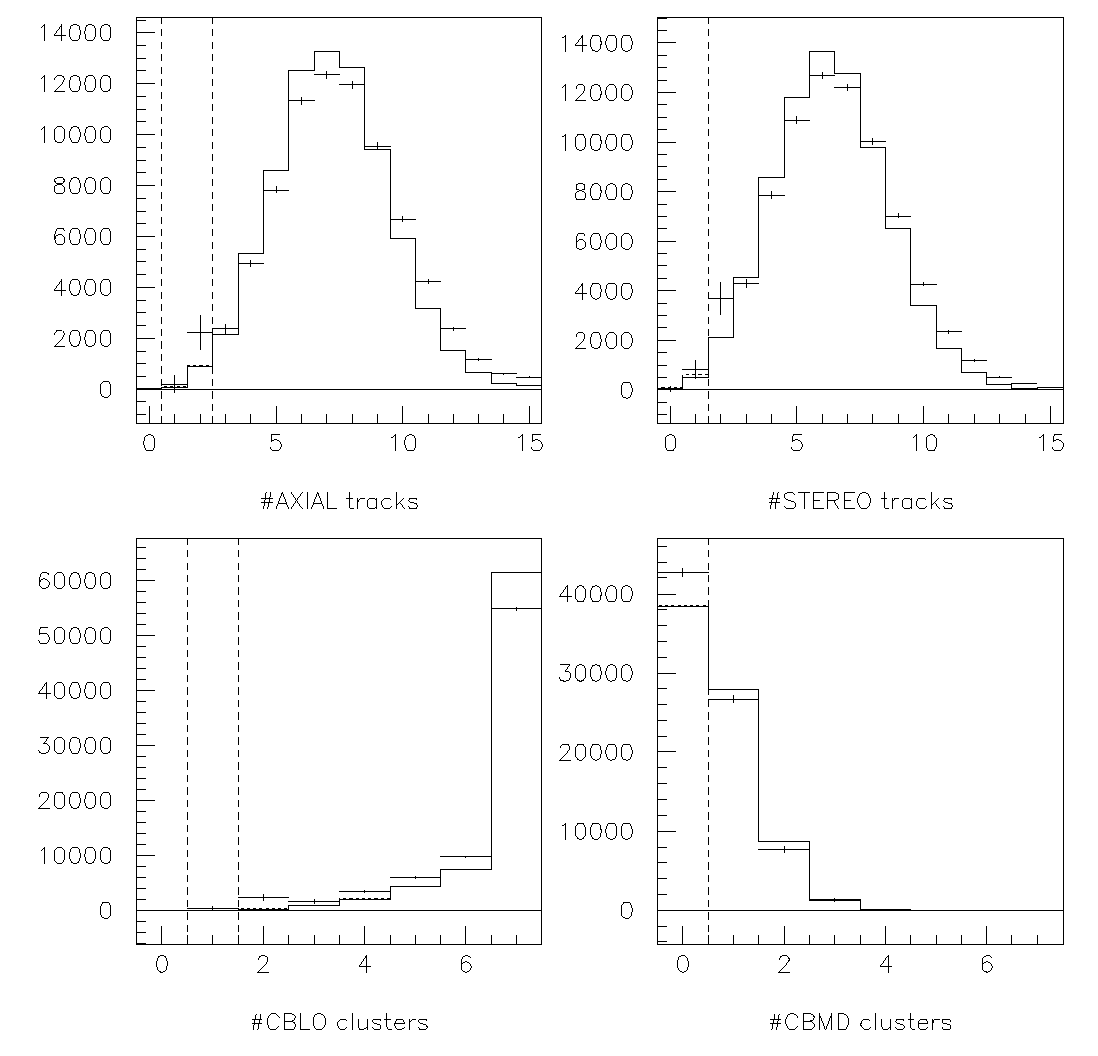
\includegraphics[width=\linewidth]{plots/trigger_lowlevel_1s}
  \end{center}
  \caption{\label{trigger_lowlevel_1s} Low-level trigger variables for
    $\Upsilon(1S)$ hadronic decays passing the trigger, from data
    (cross-hairs) and Monte Carlo (histograms).  Dashed lines indicate
    cut thresholds, and dotted histograms are Monte Carlo without the
    trigger cut.}
\end{figure}

\begin{figure}[p]
  \begin{center}
    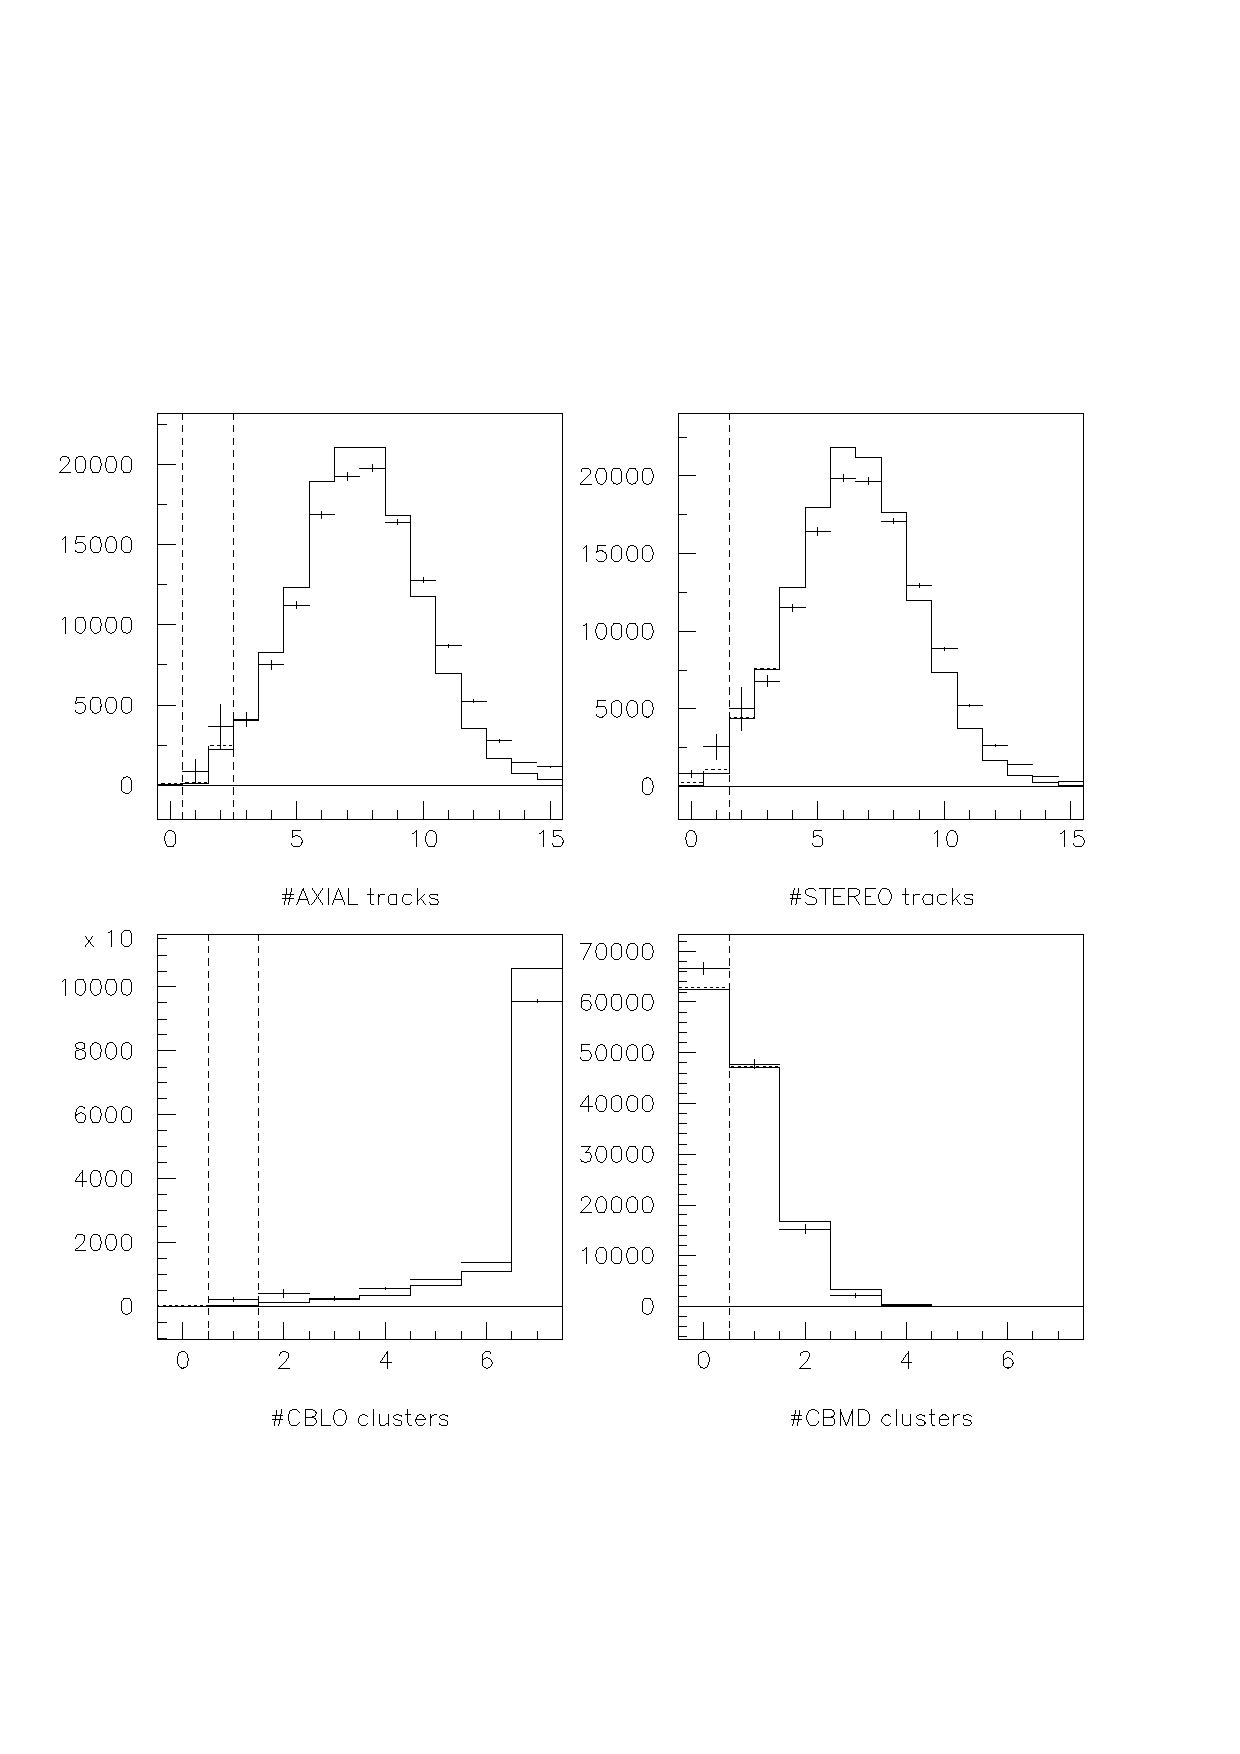
\includegraphics[width=\linewidth]{plots/trigger_lowlevel_2s}
  \end{center}
  \caption{\label{trigger_lowlevel_2s} Low-level trigger variables for
    $\Upsilon(2S)$ hadronic decays passing the trigger, from data
    (cross-hairs) and Monte Carlo (histograms).  Dashed lines indicate
    cut thresholds, and dotted histograms are Monte Carlo without the
    trigger cut.}
\end{figure}

\begin{figure}[p]
  \begin{center}
    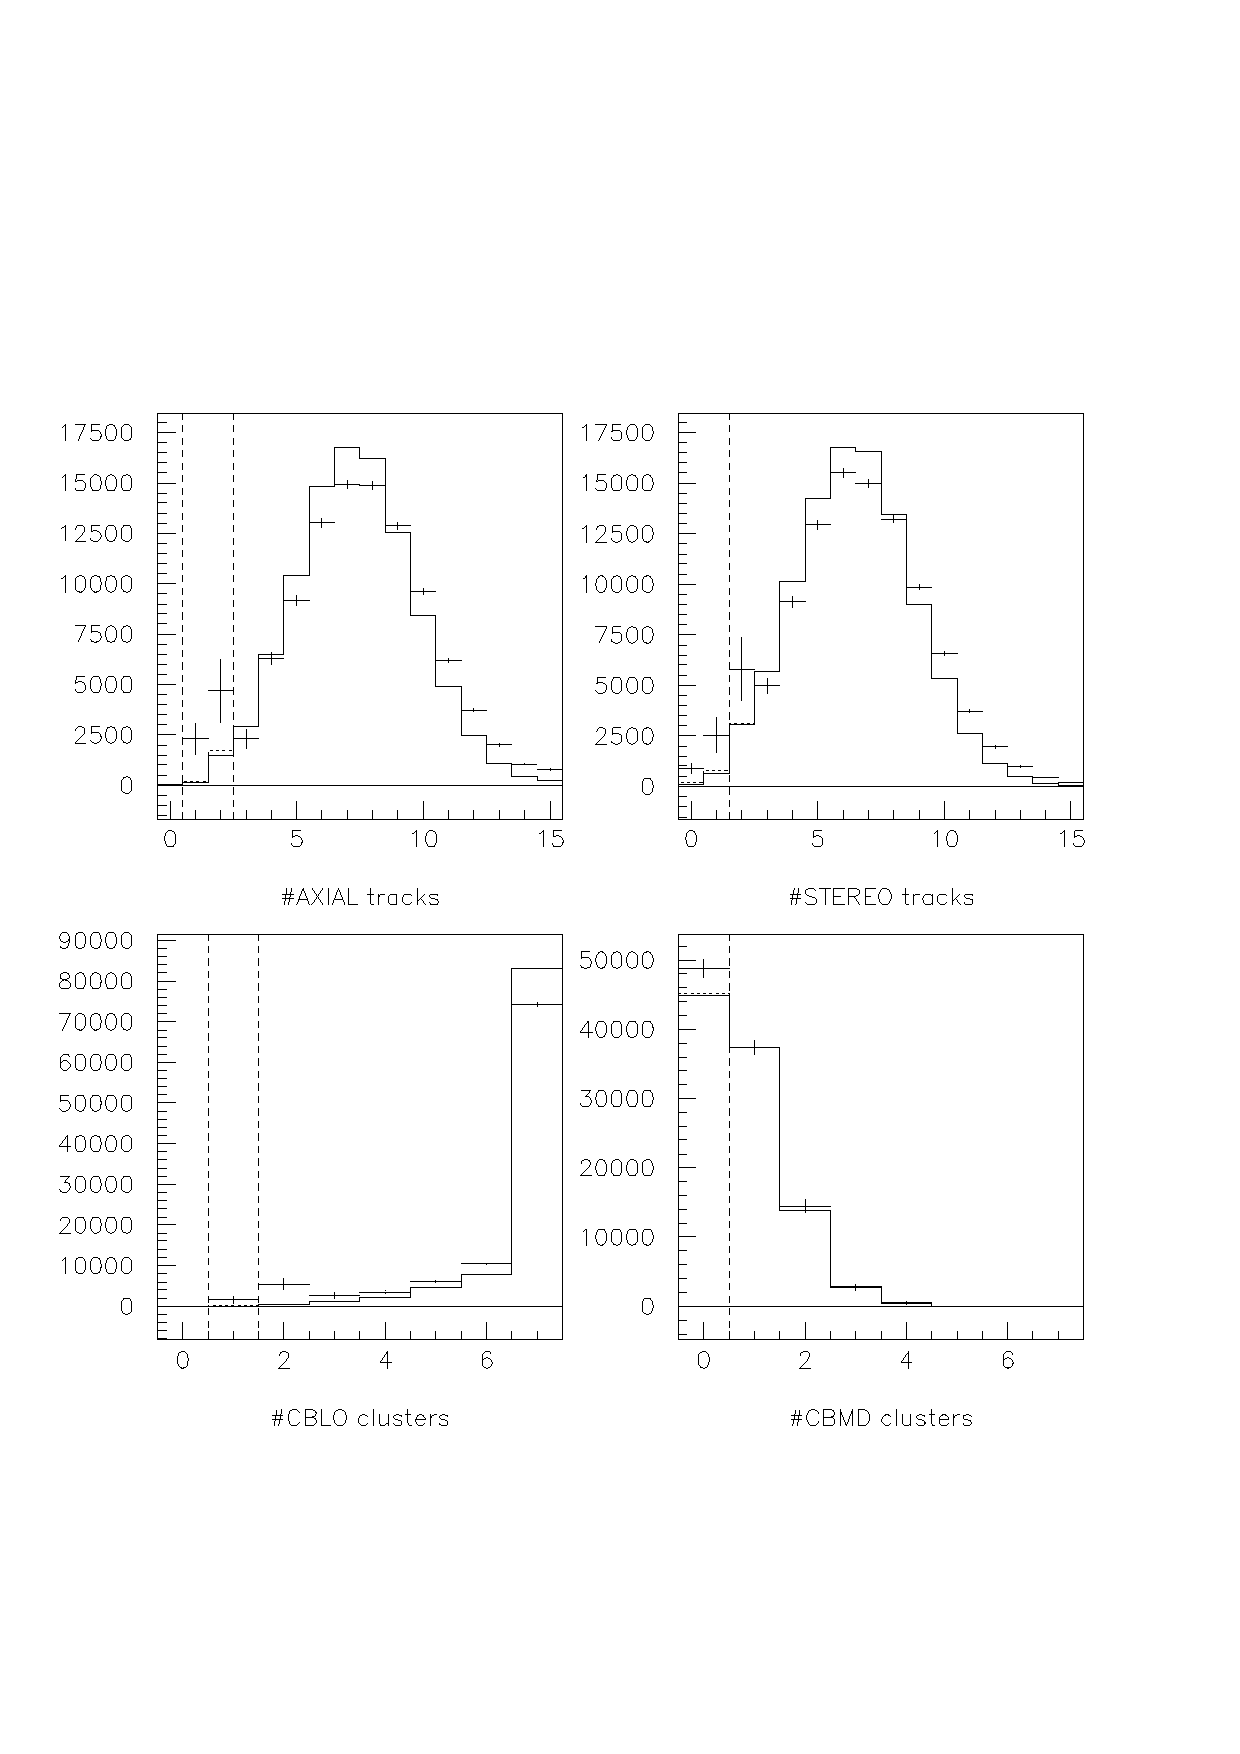
\includegraphics[width=\linewidth]{plots/trigger_lowlevel_3s}
  \end{center}
  \caption{\label{trigger_lowlevel_3s} Low-level trigger variables for
    $\Upsilon(3S)$ hadronic decays passing the trigger, from data
    (cross-hairs) and Monte Carlo (histograms).  Dashed lines indicate
    cut thresholds, and dotted histograms are Monte Carlo without the
    trigger cut.}
\end{figure}

Four discrepancies are apparent: the number of tracks distribution is
wider and higher in data, there are more CBLO clusters in the Monte
Carlo (7 is an overflow bin), there are fewer zero-CBMD events in the
Monte Carlo, and the $\Upsilon(1S)$ and $\Upsilon(3S)$ also have fewer
two-CBLO events in the Monte Carlo.

The number of quality tracks distributions in cascade data and cascade
Monte Carlo have the same discrepancy as the one seen here (Figure
\ref{cascades_tracks}), so the error is more likely to be due to the
generator's charged multiplicity distributions than modeling of DR hit
response.

The CC cluster discrepancies may all be symptoms of incorrectly
simulating the way a Monte Carlo shower is partitioned into tiles.
The two-CBLO bin, in data, is highly correlated with \#CBMD in such a
way that indicates that many showers are on the border between being
recognized as one CBMD or two CBLO.  This same correlation is present
in the Monte Carlo, but to a much lesser degree, which accounts for
both the zero-CBMD bin and the two-CBLO bin being low.  The Monte
Carlo's overestimate of \#CBLO may be due to the same error.

However, these discrepancies are easily overwhelmed by the systematic
errors I have already placed on the trigger efficiency.  Considering
that the trigger inefficiency, as measured in Monte Carlo, is 0.2\%
and 0.4\% (for the $\Upsilon(1S)$, and for the $\Upsilon(2S)$ and
$\Upsilon(3S)$, respectively), the errors I have assumed are
approximately three times the size of the effect.  The advantage of
the complete study is that I have been able to account for the
possibility that the Monte Carlo isn't simply missing a large source
of inefficiency.  Because these comparisons with data must be done
after the trigger has already filtered the events, such a possibility
could sneak through a simple data--Monte Carlo comparison.

\section{Efficiency of the Trigger for Event Type Gamgam}

Unlike hadronic decays of the $\Upsilon$, where the completeness of
the Monte Carlo has to be checked, gamgams are theoretically
well-understood.  This gives me freedom to measure gamgam cut
efficiencies in any order, so I choose to measure the trigger
efficiency after all other cuts have been applied.

My gamgam count is not going to be used to determine the total
integrated luminosity of all scans, but the integrated luminosity
ratios from one run to another.  Therefore, I am only interested in
how gamgam's trigger efficiency changes from run to run.  This is not
something I can learn from the Monte Carlo; I will need to find a way
to derive this information from the data.

BarrelBhabha, the trigger used for gamgams, requires two CBHI
clusters, one on either side of the CC barrel (one on the east and one
on the west).  There is also a very weak $\phi$ back-to-back
requirement, but it is easily satisfied by my events, especially after
I impose a strict back-to-back requirement.  BarrelBhabha suffers an
inefficiency at $\cot\theta$ = 0 (the center of the barrel) because
both CBHI clusters may be detected on the same side of the CC barrel,
due to measurement error.  This can be hard to predict, so I avoid
that region with a $|\cot\theta|$ minimum.

As its name suggests, bhabhas also satisfy the BarrelBhabha trigger.
This allows me to measure the trigger efficiency by collecting bhabhas
on a different trigger line (Hadron or RadTau or ElTrack) and then
asking if the bhabha event also satisfies BarrelBhabha.  The event
selection for bhabhas depends almost entirely on tracking
requirements, and the ElTrack trigger line is independent of
BarrelBhabha systematics inasmuch as tile inefficiencies don't appear
symmetrically on both sides of the detector.  To measure trigger
efficiency given the other gamgam cuts, each bhabha event is
additionally subjected to all gamgam cuts except
\begin{itemize}
  \item BarrelBhabha trigger line,
  \item zero quality tracks, and
  \item $|\sin(\phi_1 - \phi_2)|$ $<$ 0.04 (showers back-to-back
    in $\phi$).
\end{itemize}
The last requirement is only satisfied by particles that don't bend in
the detector's magnetic field.  The $\phi$ back-to-backness of bhabhas
is limited by a cut on \eisr.

An initial measurement of BarrelBhabha trigger efficiency revealed
holes in $\theta$ and $\phi$ that were present for different run
periods.  These holes were excluded in the gamgam cuts (and,
subsequently, the bhabhas which are used to measure BarrelBhabha
efficiency).  These are the first two ``reject'' lines in gamgam's
definition in Table \ref{cuts:eventtypes}.  A third region was
rejected because Surik Mehrabyan discovered a pair of mis-mapped
cables, which were later fixed (this could, in principle, affect the
trigger efficiency measurement).  With these restrictions, almost all
efficiencies are now 99.8\%.  Eleven outliers were investigated in the
CLEO-III e-log: most of them had ``CC trigger stripes in phi''
comments.  I have rejected these runs and listed them in Table
\ref{datasets:badruns} as having ``gamgam trigger issues.''  The final
plot of trigger efficiency versus run is in Figure
\ref{trigger_gamgam_vrun}.

The scatter in this plot is almost entirely due to statistical error.
If the number of standard deviations from the mean are plotted in a
histogram (a ``pull'' distribution, Figure \ref{trigger_gamgam_hist}),
the Gaussian width is 1.12.  The uncertainties in hadronic
cross-section will be dominated by the gamgam count, not the bhabha
correction (because bhabhas far outnumber gamgams), so there is no
harm in leaving this correction in.

\begin{figure}[p]
  \begin{center}
    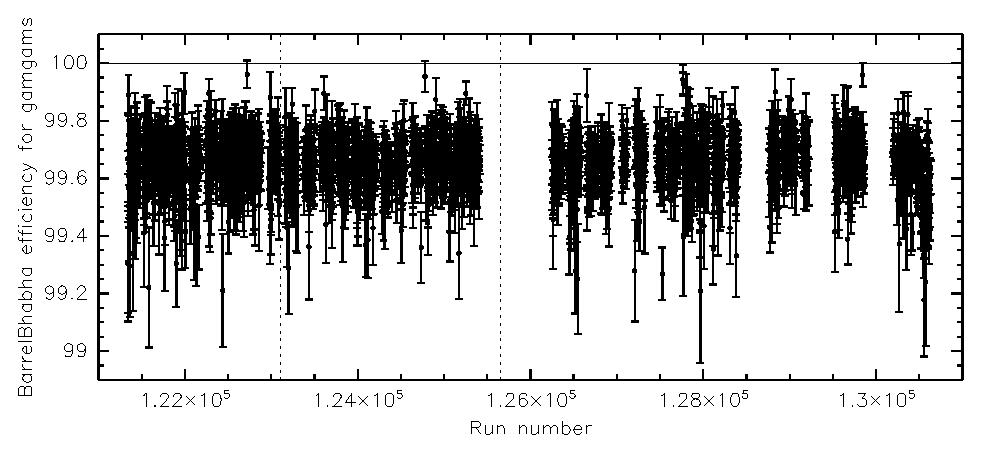
\includegraphics[width=\linewidth]{plots/trigger_gamgam_vrun}
  \end{center}
  \caption{\label{trigger_gamgam_vrun} BarrelBhabha trigger efficiency
  for gamgams, given gamgam cuts.  Dotted lines separate
  $\Upsilon(3S)$, $\Upsilon(1S)$, and $\Upsilon(2S)$ (from left to
  right).}
\end{figure}

\begin{figure}[p]
  \begin{center}
    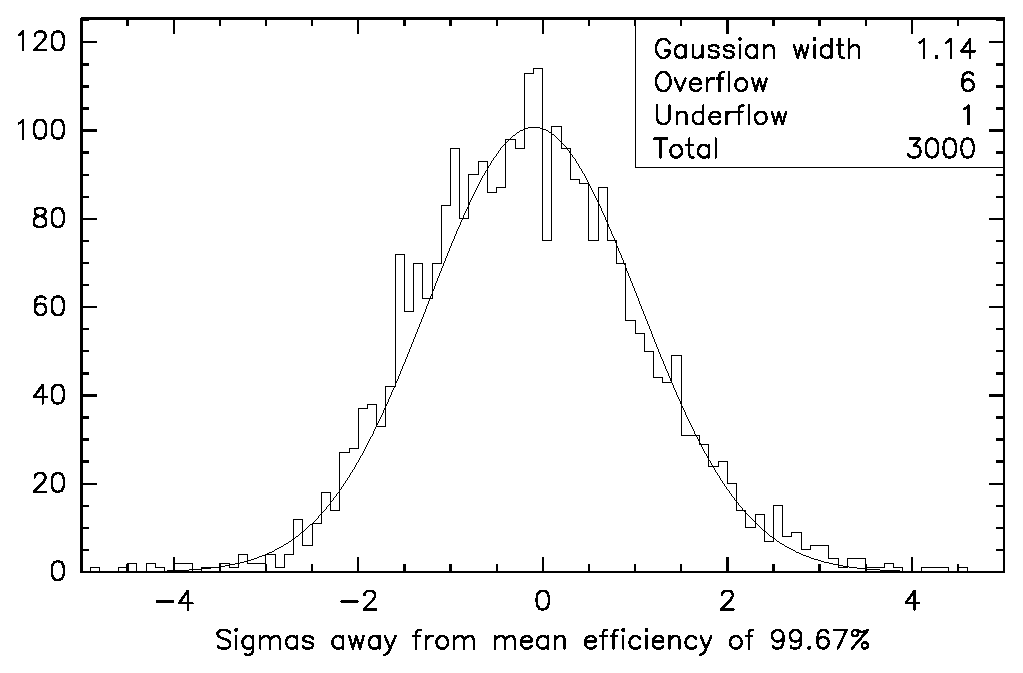
\includegraphics[width=\linewidth]{plots/trigger_gamgam_hist}
  \end{center}
  \caption{\label{trigger_gamgam_hist} Standard deviations from
    average BarrelBhabha efficiency in number of sigmas (pull
    distribution).  Each entry is a run from the database dataset.}
\end{figure}
